\documentclass[conference]{IEEEtran}
\IEEEoverridecommandlockouts
% The preceding line is only needed to identify funding in the first footnote. If that is unneeded, please comment it out.
\usepackage{cite}
\usepackage{amsmath,amssymb,amsfonts}
\usepackage{algorithmic}
\usepackage[hidelinks]{hyperref}
\usepackage[noabbrev,capitalize]{cleveref}
\usepackage{array, booktabs, makecell}
\usepackage{graphicx}
\usepackage{textcomp}
\usepackage{xcolor}
\usepackage{caption}
\usepackage{subcaption}
\newcommand\norm[1]{\left\lVert#1\right\rVert}
\def\BibTeX{{\rm B\kern-.05em{\sc i\kern-.025em b}\kern-.08em
    T\kern-.1667em\lower.7ex\hbox{E}\kern-.125emX}}
\newcommand{\red}[1]{\textcolor{red}{#1}}

\graphicspath{../}
\hypersetup{
    colorlinks=true,
    linkcolor=black,
    filecolor=black,      
    citecolor=black,
    urlcolor=blue,
    pdfpagemode=FullScreen,
    }

\begin{document}

\title{An Indirect, Multiscale and Robust Approach to Global Motion Estimation}

\author{\IEEEauthorblockN{Filippo Daniotti}
\IEEEauthorblockA{\textit{DISI, University of Trento} \\
Trento, Italy\\
filippo.daniotti@studenti.unitn.it\\
232087}
\and
\IEEEauthorblockN{Samuele Conti}
\IEEEauthorblockA{\textit{DISI, University of Trento} \\
Trento, Italy\\
samuele.conti@studenti.unitn.it\\
229294}
}

\maketitle

% add page number
\thispagestyle{plain}
\pagestyle{plain}

\begin{abstract}
The problem of global motion estimation (GME) deals with the separation, in a video sequence, of two different types of motion: the \emph{egomotion} of the camera recording the video, and the actual motion of the objects recorded. The literature presents a number of possible approaches to the GME problem; here, we aim to combine some of the most effective strategies to compute the motion of the camera. We adopt an indirect approach based on a perspective motion model (as \cite{Dufeaux2000}). Following a multi-resolution approach, at the lower-resolution level, we use block matching estimation to get a dense motion field; then, at each following (higher-resolution) level we optimize the current parameters of the motion model with gradient descent. During the process of gradient descent the outliers are discarded, in order to get a robust estimation. The final result consists in the optimized list of parameters of the motion model.  
\end{abstract}

\begin{IEEEkeywords}
multi-resolution, robust, indirect, global motion estimation, computer vision, video processing
\end{IEEEkeywords}

\section{Introduction}
\label{sec:01-intro}
The problem of global motion estimation (GME) deals with the separation, in a video sequence, of two different types of motion: the egomotion of the camera capturing the video, and the actual motion of the objects in the scene. This task is crucial for a number of application, for instance:
\begin{itemize}
    \item removal of camera shaking or noisy motion;
    \item study of the motion of the camera itself;
    \item object segmentation and recognition;
    \item object tracking.
\end{itemize}

For these reasons, motion estimation is a problem that has long been studied, hence in the literature we can find a variety of approaches to the problem. In this work we concentrated on some of the most effective approaches and combined them to get an indirect, multi-resolution and robust approach to GME.

The document is structured as follows: in Sec.\ref{sec:02-gme} we sum up the fundamental aspects of the GME problem and the standard approaches to solve these problems. In Sec.\ref{sec:03-implementation} we discuss the strategies we chose for our implementation, and in Sec.\ref{sec:04-results} we present the results of this work. The conclusions in Sec.\ref{sec:conclusions} sum up the work and draw a path for future development.

\section{Global Motion Estimation}
\label{sec:02-gme}
When we look at a video, which corresponds to a sequence of images, called frames, we can spot the movement between one frame and the other by detecting the pixels that changed position with respect to the pair of frames.

This information can be encoded in a human-understandable format by presenting the needle diagram of the two frames; this kind of representation is shown in \cref{fig:needle-diagram}. 

\begin{figure}
    \centering
    \includegraphics[width=.7\linewidth]{../assets/images/bbme-0-res.png}
    \caption{Needle diagram between two frames of a video sequence.}
    \label{fig:needle-diagram}
\end{figure}

The message of the figure is pretty clear: for each couple of frames we mark with an arrow the shift that the pixel has made. This gives us an indication of the actual movement of the recorded objects.

But the movement that we are able to extract from the two frames is what is usually called "apparent motion", which is a combination of two different factors:
\begin{itemize}[noitemsep]
    \item the global motion, which corresponds with the motion of the camera;
    \item the effective motion of the objects recorded.
\end{itemize}

An important task in computer vision is the global motion estimation, which corresponds to being able to distinguish these two different motions.
As stated in the abstract, this information is highly important for a number of applications, among which we find video coding, motion compensation and egomotion estimation.

But the task of distinguishing which movement is to be classified as global motion and which one is to be classified as object motion instead is not so easy. In fact, there is no clear feature that distinguishes the moving objects from the static background, and this leads to the need for complex tools to differentiate the two typed of motion.

The main approach to global motion estimation consists in ...


As \cite{Dufeaux2000}
\section{Implementation choices}
\label{sec:03-implementation}
Describe the choices with links to the previous section.
Insert pseudocode of the implementation.

As stated in \cref{sec:motion-models}, we decided to use an indirect method with affine model for motion estimation as in Bergen et al.\cite{Bergen92}; also, we decided to obtain a robust estimation by using a strategy similar to Dufaux and Konrad\cite{Dufeaux2000}, where they adopt a hierarchical approach to obtain a robust estimation using coarse resolution to guide the search for the best parameters at a finer resolution.

In the following sections, we will provide an in-depth explaination of our solution and present the pseudocode of the algorithm. A schematic representation of the procedure is presented in \cref{fig:gme-schema}.

\begin{figure}
    \centering
    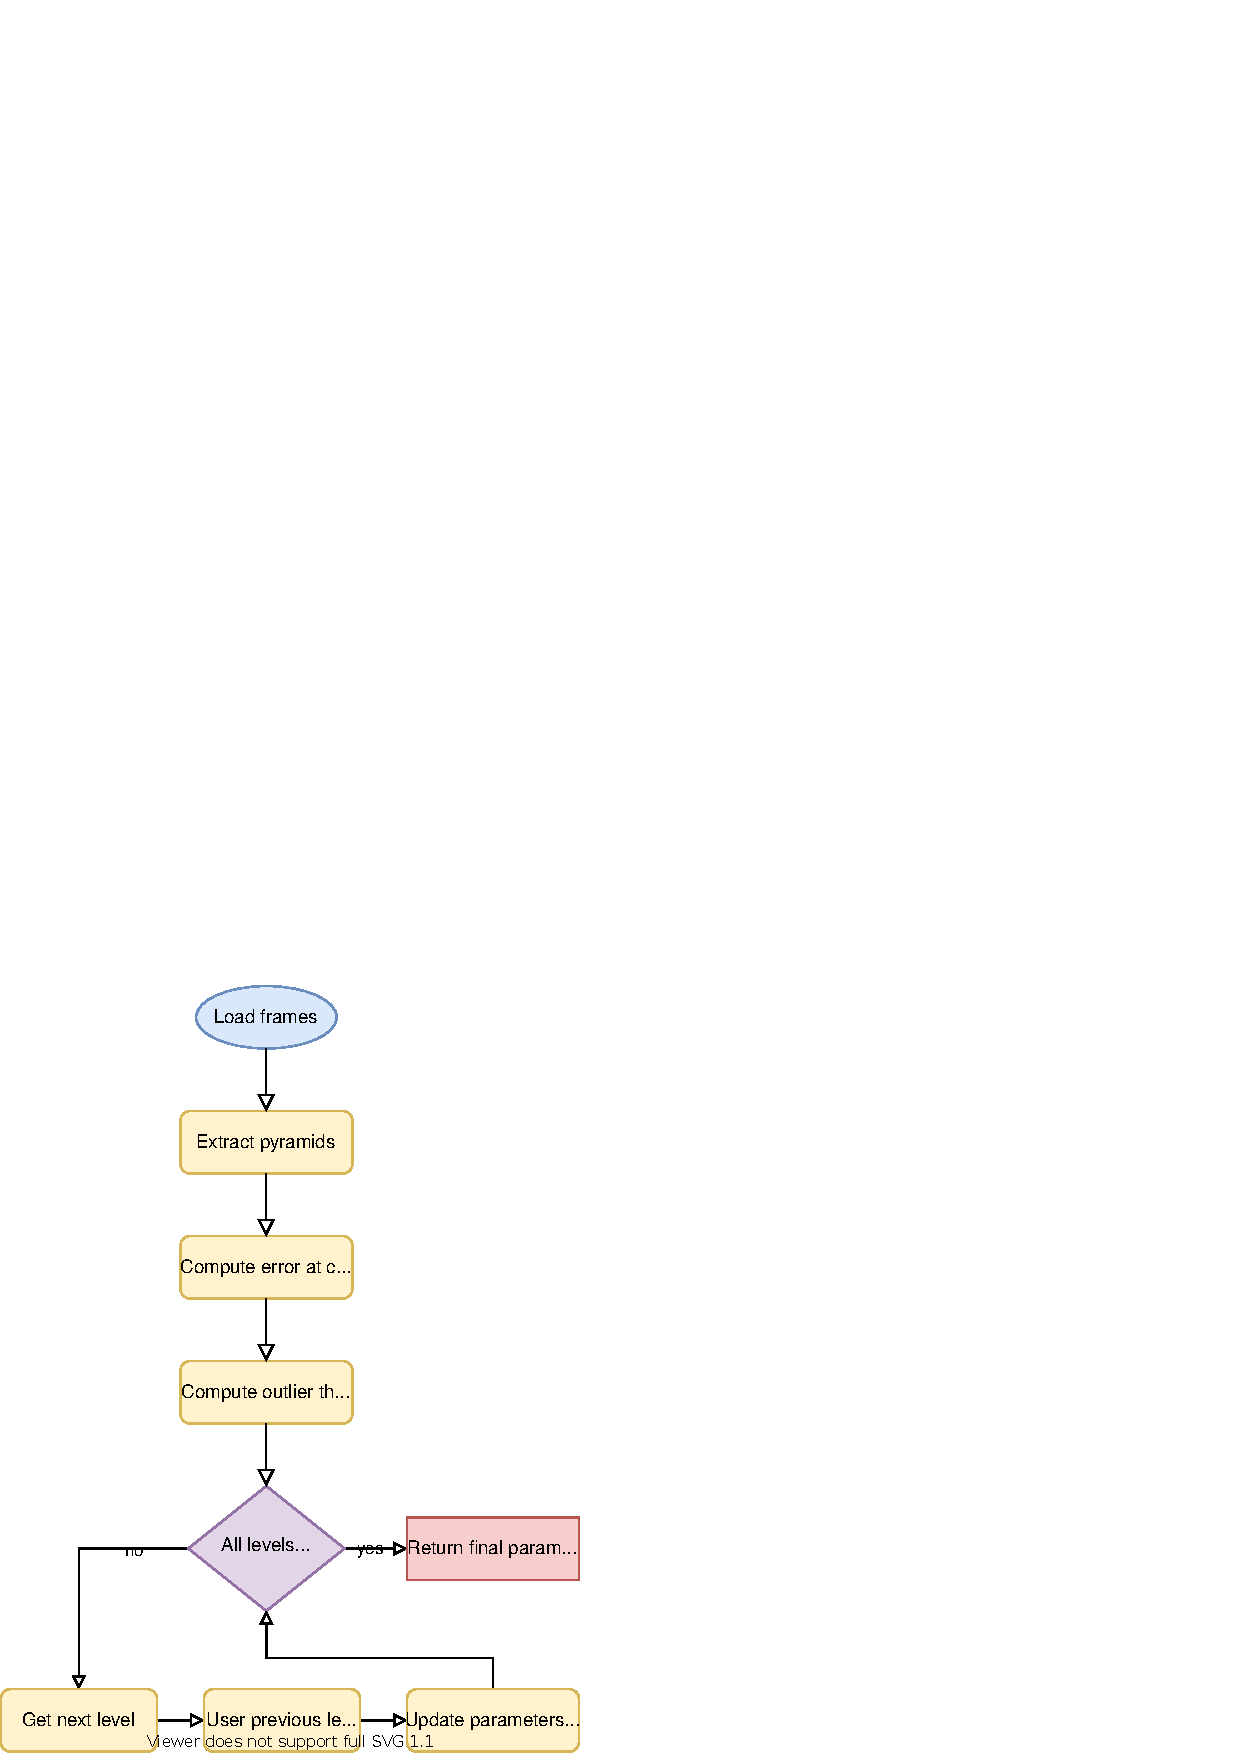
\includegraphics[width=.7\linewidth]{../assets/images/implementation-flow.png}
    \caption{Schema of the flow of implementation of the global motion estimation pipeline.}
    \label{fig:implementation-flow}
\end{figure}

\subsection{Block-Based Motion Estimation}
\label{sec:BBME}
The first piece of the architecture is the algorithm to compute the motion field to be used as ground truth.
In our case, we decided to implement a block matching motion estimation (BBME), as computing the motion field on blocks, rather than single pixels, can be much less computationally expensive.

The main idea of BBME is to divide the frame in blocks, and search for each block in the previous frame the corresponding block in the next frame.
This gives us the displacement of the block between the two frames, which is treated as the motion vector of the block.
This is the basic principle of BBME, from which derived a number of implementations that present differences mainly in two aspects:
\begin{enumerate}
    \item the size and shape of the block;
    \item the path that the searching procedure follows.
\end{enumerate}

During the project we implemented a number of these techniques:
\begin{itemize}
    \item exhaustive search;
    \item two-dimensional logarithmic search;
    \item \blue{new} three-step search, from \cite{Li94};
    \item diamond search, from \cite{Zhu2000};
\end{itemize}

In the final implementation, the block matching method used is the one presented in \cite{Zhu2000}, known as diamond search (DS),  with a mean square error measure to compute (dis-)similarity between blocks.
Nonetheless, all the other methods are still present and by slightly changing the code they can be tested as well.

Here we briefly discuss the algorithm that we choose to implement and propose a small example for clarification.
The DS algorithm uses a peculiar diamond-shaped search pattern, which defines which positions will be used as target points where to center the block in the next frame to see if it corresponds to the block in the previous frame. In particular, the algorithm uses two slighlty different shapes depending on the current iteration (see \cref*{fig:ds-search-patterns}):
\begin{itemize}
    \item large diamond search pattern;
    \item small diamond search pattern.
\end{itemize}

\begin{figure}
    \centering
    \includegraphics[width=.95\linewidth]{../assets/images/ds-search-patterns.png}
    \caption{Representation of the two DS algorithm search patterns}
    \label{fig:ds-search-patterns}
\end{figure}

The procedure is the following:
\begin{enumerate}
    \item the search starts with LDSP, meaning that we check the blocks centered in each one of the 9 positions; if the best match is the central position then we pass to the second step, otherwise we move to the best match position and re-use the LDSP;
    \item in the second step we use SDSP and look again for the best matching position among the 5 available, then return the best match position.
\end{enumerate}

\begin{figure}
    \centering
    \includegraphics[width=.95\linewidth]{../assets/images/ds-exe.png}
    \caption{Example of run of diamond search algorithm for block matching motion estimation.}
    \label{fig:diamond-search-example}
\end{figure}

In \cref{fig:diamond-search-example} we can see an example of run. We can spot the three large-shape diamonds (the contour position are marked with circles) and the small shaped diamond (contour positions marked with triangles).
In this example the block matching algorithm started from $\{0,0\}$, then moved with the large diamond to $\{-2,0\}$, because this was the position that minimized the error between the block in the previous and the next frame. Then again with the large diamond the algorithm reached $\{-3,-1\}$ first, and $\{-4,-2\}$ after. Here the best matching position for the large diamond shape was $\{-4,-2\}$, therefore the algorithm stopped using the large diamond and started with the small diamond. Finally, the small diamond returned once again as best match position $\{-4,-2\}$, which was then returned as final matching position for the block in the previous frame.

\subsection{Affine Model Parameter Estimation}
In \cref{sec:motion-models}, we presented the affine motion model, which is the one we decided to use in our implementation.

To get the motion vector of a certain position $\{x,y\}$ in the previous frame, we can solve the following formulation of the affine model:
\begin{equation}
    \label{eq:displacement-matrix-formulation}
    d(p, a) = A(p)\;a
\end{equation}
where $d(p, a)$ is the displacement for the position $p = \{x,y\}$, given the parameter vector $a$; $A(p)$ is an intermediate matrix that is computed as 
\begin{equation*}
    A(p) = \begin{bmatrix}
        1 & x & y & 0 & 0 & 0 \\
        0 & 0 & 0 & 1 & x & y
    \end{bmatrix}
\end{equation*}

By encoding the estimation of the motion field in this way, the $p$-norm error we are trying to minimize (see \cref{eq:indirect-estimation}), gets rewritten in this way:

\begin{equation}
    \label{eq:pnorm-error}
    E = \sum_p{\left| d(p, a) - d(p) \right|^P}
\end{equation}
Here we introduce $d(p)$ as the ground truth motion vector (the one we get from the BBME as in \cref{sec:BBME}) and $P$ which specifies the grade of the $p$-norm used. In this case we decided to set $P=2$, following the procedure explained in \cite{WangBook}.
\blue{why do you use capital P tho}

The next step is to minimize the error in \cref{eq:pnorm-error} with respect to the parameter vector $p$.
The procedure in \cite{WangBook} states that we need to compute the gradient of $E$ w.r.t $p$, and then get the value of $p$ that sets the gradient to 0.

By using the matrix formulation explained in \cref{eq:displacement-matrix-formulation} and by setting the gradient $\nabla_a E = 0$, we obtain the following result:
\begin{equation}
    \label{eq:optimal-parameter-affine}
    a = \left (\sum_p A(p)^T A(p) \right )^{-1} \left (\sum_p A(p)^T d(x) \right)
\end{equation}

There are three interesting notes about \cref{eq:optimal-parameter-affine}:
\begin{enumerate}
    \item we are iterating over a set of positions $p$: it's interesting to notice that these points do not need to cover the complete scene, i.e. we can use only a subset of the image to optimize the parameters;
    \item each one of the points can be weighted with a weight $w(p)$ as shown in \cref{eq:optimal-parameter-affine-weighted};
    \item we can actually split the computation of the parameter vector $a = [a_1, a_2, a_3, b_1, b_2, b_3]$ in two different slices, $a_x = [a_1, a_2, a_3]$ and $a_y = [b_1, b_2, b_3]$, which can be computed in a specular way as shown in \cref{eq:optimal-parameter-affine-weighted-halved} this is useful to further reduce the complexity of the procedure.
\end{enumerate} 

\begin{equation}
    \label{eq:optimal-parameter-affine-weighted}
    a = \left (\sum_p w(p) A(p)^T A(p) \right )^{-1} \left (\sum_p w(p) A(p)^T d(x) \right)
\end{equation}

\begin{equation}
    \label{eq:optimal-parameter-affine-weighted-halved}
    a_x = \left (\sum_p w(p) A_x(p)^T A_x(p) \right )^{-1} \left (\sum_p w(p) A_x(p)^T d_x(x) \right)
\end{equation}
where $A_x(p) = [1,x,y]$.

The form of the solution that we used in the implementation is the one reported in \cref{eq:optimal-parameter-affine-weighted-halved}.

\subsection{Hierarchical Robust Estimation}
There is still one last strategy employed in the project, which is used to provide a robust estimation of the parameters for the affine motion model.

The strategy employed here takes inspiration from \cite{Dufeaux2000}, where the computation of the motion field takes place at different levels of resolution. The idea is to exploit the computation at a coarser resolution to extract information useful for regularizing the estimation at finer resolutions.

\section{Results}
\label{sec:04-results}

\subsection{Qualitative results}
The easiest and most effective way to show the results of a global motion estimation pipeline is to use qualitative information, as  the reader will understand it straightforwardly.

One of the operations that shows intuitively the implications of global motion estimation is camera motion compensation. 
In short, if the video is recorded by a camera which is moving, we will see the two types of motion explained in \cref{sec:01-intro}: apparent and real. The aim of camera-motion compensation is to detect and remove the apparent motion which is caused only by the (ego)motion of the camera.

To show the results obtained we reported in image \cref{fig:qualitative-results} an example in which the reader can observe:
\begin{itemize}
    \item the previous frame in \cref{fig:prev-frame};
    \item the next frame in \cref{fig:curr-frame};
    \item the compensated frame, obtained by compensating camera motion in the previous frame, in \cref{fig:compensated};
    \item the absolute difference between next and previous frame in \cref{fig:diff-curr-prev}, which gives an idea of how strong the motion in which parts of the image is;
    \item the motion field generated by the camera, as returned by our estimation procedure in \cref{fig:est-mf};
    \item the absolute difference between the next frame and the compensated one in \cref{fig:diff-curr-comp}.
\end{itemize}

\begin{figure*}[!h]

    \begin{subfigure}[b]{0.3\textwidth}
        \centering
        \includegraphics[width=1\textwidth]{../assets/images/pan240-prev-frame.png}
        \caption{Previous frame.}
        \label{fig:prev-frame}
    \end{subfigure}
    \hfill
    \begin{subfigure}[b]{0.3\textwidth}
        \includegraphics[width=1\textwidth]{../assets/images/pan240-curr-frame.png}
        \caption{Next frame.}
        \label{fig:curr-frame}
    \end{subfigure}
    \hfill
    \begin{subfigure}[b]{0.3\textwidth}
        \includegraphics[width=1\textwidth]{../assets/images/pan240-compensated.png}
        \caption{Compensated previous frame.}
        \label{fig:compensated}
    \end{subfigure}
    
    \vspace{0.5em}

    \begin{subfigure}[b]{0.3\textwidth}
        \centering
        \includegraphics[width=1\textwidth]{../assets/images/pan240-diff-curr-prev-1.png}
        \caption{Absolute difference between current and previous frame (white areas are where we detect motion).}
        \label{fig:diff-curr-prev}
    \end{subfigure}
    \hfill
    \begin{subfigure}[b]{0.3\textwidth}
        \includegraphics[width=1\textwidth]{../assets//images/pan240-camera-motion-1.png}
        \caption{Global motion field estimated by our procedure, it corresponds to the motion generated by the camera.}
        \label{fig:est-mf}
    \end{subfigure}
    \hfill
    \begin{subfigure}[b]{0.3\textwidth}
        \includegraphics[width=1\textwidth]{../assets/images/pan240-diff-curr-comp.png}
        \caption{Absolute difference between current and compensated frame, the only object in white is the only actually moving.}
        \label{fig:diff-curr-comp}
    \end{subfigure}

    \caption{Qualitative results.}
    \label{fig:qualitative-results}
\end{figure*}

\paragraph{How to interpret qualitative results} We should be able to notice in the results that the motion that we detect between the two frames (previous and next) is significantly large and noticeable. In fact, by using the absolute difference between frames, we can see that a big part of the visual field seems to be moving in \cref{fig:diff-curr-prev}.

However, by computing the motion generated by the camera egomotion, we find out that most of the shift we register is apparent.
By estimating the motion generated by the camera, which is reported in  \cref{fig:est-mf}, we can compensate the apparent motion in the previous frame.
When we compensate the previous frame we \textit{remove} all the motion due to apparent motion; therefore, if we compare the current frame and the compensated frame (see \cref{fig:diff-curr-comp}) we are able to isolate real motion.

The results shown are consistent since the video from which the frames are taken was recorded with the camera moving in the horizontal direction while the person in the video was walking.

\subsection{Quantitative results}

To perform a numeric quantitative analysis of the results produced by the algorithm we used, once again, the compensation of the previous frame. Put it simply, in a video sequence where there is no real motion, but only camera motion, the compensation of the apparent motion should be enough to make the current and the compensated frame identical.

Therefore, in \cref{tab:psnr}, we present some PSNR values for different video sequences. We annotated the table with some considerations about the videos, as PSNR value is influenced also by properties of the video like the strength of motion or the presence/absence of real motion.

For instance, in the case where there are medium or big objects, like the last two entries of the table, the PSNR turns out to be low, since the model is not able to distinguish between object and camera motion.

Better results can be observed in the first two entries of the table, where the moving object are considerably smaller with respect to the background, and the background presents some complex pattern, which enables the algorithm to better detect its motion.

\begin{table*}[!t]
    \begin{center}
        \begin{tabular}{ll|rrrr}
        \toprule
        Video & Properties & Average & Variance & Maximum & Minimum \\
        \midrule
        \texttt{pan240.mp4} & Fast motion & \(22.724\)  & \(5.125\)  & \(27.802\) & \(17.981\)  \\
        
        \texttt{coastguard\_qcif.mp4} & Two object moving, background moving & \(22.733\)  & \(2.194\)  & \(26.875\) & \(15.158\)  \\
        
        \texttt{foreman.mp4} & Big object moving, still background & \(19.677\)  & \(18.443\)  & \(30.436\) & \(11.746\)  \\
        
        \texttt{numeri\_del\_piero.mp4} & Medium object moving, moving background & \(19.072\)  & \(13.642\)  & \(47.722\) & \(16.323\)  \\
        \bottomrule
    \end{tabular}
    \caption{PSNR results on some meaningful video samples.}
    \label{tab:psnr}
\end{center}
\end{table*}    
\section{Conclusions}
\label{sec:conclusions}

This project addresses the task of global motion estimation through the use of an indirect method for the estimation of apparent motion which is based on the affine motion model.

During the implementation of the tool, we built the following scripts:
\begin{itemize}
    \item \texttt{bbme.py} as Python module containing all the functions related to the various block matching motion estimation procedures that we tried;
    \item \texttt{motion.py} as Python module containing all the functions (and constants) needed in order to perform camera motion estimation and motion compensation;
    \item \texttt{results.py} as example of use of the packages modules to produce the results we used also to create this report.  
\end{itemize}

The approach we used proved to be efficient and robust, as long as the motion in the image is not too complex and as long as the background is not uniform and, therefore, the BBME algorithms are able to spot its motion.

The actual implementation is to be found in the following GitHub repository \url{https://github.com/Samaretas/global-motion-estimation}, where the reader can find all the commented scripts and try out the code.
In the repository it will be possible to run the basic example with \texttt{pan240.mp4}, whether the other videos of the dataset can be found here \url{https://drive.google.com/drive/folders/1gZisWe4DEWpb_CoHkTi6OKnxhl5Ca_mT?usp=sharing}.

For more information on the code and how to perform a full-cycle execution of the pipelen, please refer to the Github repository.

\bibliography{bibliography.bib}{}
\bibliographystyle{IEEEtran}

\end{document}
